%% LyX 2.5.1 created this file.  For more info, see https://www.lyx.org/.
%% Do not edit unless you really know what you are doing.
\documentclass[12pt,english]{article}
\usepackage[utf8]{inputenc}
\usepackage{babel}
\usepackage{xr}
\usepackage{mathrsfs}
\usepackage{mathtools}
\usepackage{amsmath}
\usepackage{amsthm}
\usepackage{amssymb}
\usepackage{geometry}
\geometry{verbose}
\usepackage[bookmarks=false,
 breaklinks=false,pdfborder={0 0 1},backref=false,colorlinks=false]
 {hyperref}

\makeatletter
\@ifundefined{date}{}{\date{}}
%%%%%%%%%%%%%%%%%%%%%%%%%%%%%% User specified LaTeX commands.
\usepackage{mathrsfs}
% also loads amsmath
\usepackage{amsfonts}\usepackage{tikz}


% \usepackage{subfig}
\PassOptionsToPackage{english}{babel}
\usepackage{babel}
% \usepackage{capt-of}
% \usepackage{tabularray}
\usepackage{caption}
\usepackage{subcaption}
% \usepackage{caption}
\captionsetup{skip=0pt}   
% \subcaptionsetup{skip=0pt}   
% \captionsetup[sub]{skip=0pt}   
% \usepackage{subcaption}
% \captionsetup{compatibility=false}
\usepackage{graphicx}
\newtheorem{theorem}{Theorem}\usetikzlibrary{calc}
\usetikzlibrary{shapes}
%might be unnecessary
% \usepackage{doi}

%bibliography CMDS

%\usepackage{cite}
%\usepackage[style=alphabetic]{biblatex}
%\bibliographystyle{plain}

%\usepackage[style=alphabetic]{biblatex}

% \usepackage[backend=biber,style=alphabetic]{biblatex}
% \usepackage[backend=biber,style=abbrv]{biblatex}
% \usepackage[backend=biber,style=alpha]{biblatex}
%\usepackage[backend=bibtex,style=alphabetic]{biblatex}


%%% With amsthm package, creates environments for nicely formatted,
%%% labeled, and numbered propositions, etc.
\theoremstyle{plain}

\newtheorem{thm}{Theorem}[section]
\newtheorem{lemma}[thm]{Lemma}\newtheorem{prop}[thm]{Proposition}\providecommand{\propositionname}{Proposition}
\newtheorem*{prop*}{\protect\propositionname}\newtheorem{conj}[thm]{Conjecture}\newtheorem{cor}[thm]{Corollary}\newtheorem{claim}[thm]{Claim}\newtheorem{fact}[thm]{Fact}\newtheorem{constraint}[thm]{Constraint}\newtheorem{condition}[thm]{Condition}\providecommand{\claimname}{Claim}
\theoremstyle{remark}
\newtheorem*{claim*}{\protect\claimname}

\theoremstyle{definition}
\providecommand{\definitionname}{Definition}
\newtheorem*{defn*}{\protect\definitionname}\newtheorem{eg}[thm]{Example}\newtheorem{definition}{Definition}[section]
\newtheorem{rem}[thm]{Remark}\newtheorem{observ}[thm]{Observation}\newtheorem{open}[thm]{Open Problem}\newtheorem{prob.}[thm]{Problem}\newtheorem{quest}[thm]{Question}

% I used these for making definitions and theorems, not what is above
\theoremstyle{remark}
\newtheorem{remark}[thm]{Remark}\newtheorem{note}[thm]{Note}

\theoremstyle{definition}
% \newtheorem{definition}{Definition}[section]
\newtheorem{exmp}{Example}[section]

%custom commands

% blank cell
\newcommand{\cell}[4]{ \draw[thick] ( #1 , #2 ) rectangle ( #3 , #4 );}

% invisible cell for spacing
\newcommand{\spacecell}[4]{ \draw[thick, color=white] ( #1 , #2 ) rectangle ( #3 , #4 );}

% open cell 
\newcommand{\cellopen}[4]{ \draw[thick] ( #1 , #2 ) rectangle ( #3 , #4 ); \node[shape=circle,draw=red,fill=red, inner sep=0pt,minimum size=3pt] (A) at ( #1 * 0.5 + #3 * 0.5 , #2 * 0.5 + #4 * 0.5 ){};}

\newcommand{\cellA}[4]{ \draw[thick] ( #1 , #2 ) rectangle ( #3 , #4 ); \draw[red, thick, densely dotted] (#3 * 0.5 + #1 * 0.5 , #2) -- (#1, #4 * 0.5 + #2 * 0.5);}
\newcommand{\cellB}[4]{ \draw[thick] ( #1 , #2 ) rectangle ( #3 , #4 ); \draw[red, thick, densely dotted] (#3 * 0.5 + #1 * 0.5 , #2) -- (#3, #4 * 0.5 + #2 * 0.5);}
\newcommand{\cellC}[4]{ \draw[thick] ( #1 , #2 ) rectangle ( #3 , #4 ); \draw[red, thick, densely dotted] (#3 * 0.5 + #1 * 0.5 , #4) -- (#3, #4 * 0.5 + #2 * 0.5);}
\newcommand{\cellD}[4]{ \draw[thick] ( #1 , #2 ) rectangle ( #3 , #4 ); \draw[red, thick, densely dotted] (#3 * 0.5 + #1 * 0.5 , #4) -- (#1, #4 * 0.5 + #2 * 0.5);}
\newcommand{\cellE}[4]{ \draw[thick] ( #1 , #2 ) rectangle ( #3 , #4 ); \draw[red, thick, densely dotted] (#3, #4 * 0.5 + #2 * 0.5) -- (#1, #4 * 0.5 + #2 * 0.5);}
\newcommand{\cellF}[4]{ \draw[thick] ( #1 , #2 ) rectangle ( #3 , #4 ); \draw[red, thick, densely dotted] (#3 * 0.5 + #1 * 0.5 , #2) -- (#3 * 0.5 + #1 * 0.5 , #4);}

\newcommand{\cellf}[4]{\filldraw[gray!80] ( #1 , #2 ) rectangle ( #3 , #4 ); \draw[thick] ( #1 , #2 ) rectangle ( #3 , #4 );}

\newcommand{\cellAf}[4]{\filldraw[gray!80] ( #1 , #2 ) rectangle ( #3 , #4 ); \draw[thick] ( #1 , #2 ) rectangle ( #3 , #4 ); \draw[red, thick, densely dotted] (#3 * 0.5 + #1 * 0.5 , #2) -- (#1, #4 * 0.5 + #2 * 0.5);}
\newcommand{\cellBf}[4]{\filldraw[gray!80] ( #1 , #2 ) rectangle ( #3 , #4 ); \draw[thick] ( #1 , #2 ) rectangle ( #3 , #4 ); \draw[red, thick, densely dotted] (#3 * 0.5 + #1 * 0.5 , #2) -- (#3, #4 * 0.5 + #2 * 0.5);}
\newcommand{\cellCf}[4]{\filldraw[gray!80] ( #1 , #2 ) rectangle ( #3 , #4 ); \draw[thick] ( #1 , #2 ) rectangle ( #3 , #4 ); \draw[red, thick, densely dotted] (#3 * 0.5 + #1 * 0.5 , #4) -- (#3, #4 * 0.5 + #2 * 0.5);}
\newcommand{\cellDf}[4]{\filldraw[gray!80] ( #1 , #2 ) rectangle ( #3 , #4 ); \draw[thick] ( #1 , #2 ) rectangle ( #3 , #4 ); \draw[red, thick, densely dotted] (#3 * 0.5 + #1 * 0.5 , #4) -- (#1, #4 * 0.5 + #2 * 0.5);}
\newcommand{\cellEf}[4]{\filldraw[gray!80] ( #1 , #2 ) rectangle ( #3 , #4 ); \draw[thick] ( #1 , #2 ) rectangle ( #3 , #4 ); \draw[red, thick, densely dotted] (#3, #4 * 0.5 + #2 * 0.5) -- (#1, #4 * 0.5 + #2 * 0.5);}
\newcommand{\cellFf}[4]{\filldraw[gray!80] ( #1 , #2 ) rectangle ( #3 , #4 ); \draw[thick] ( #1 , #2 ) rectangle ( #3 , #4 ); \draw[red, thick, densely dotted] (#3 * 0.5 + #1 * 0.5 , #2) -- (#3 * 0.5 + #1 * 0.5 , #4);}

% before and after diagrams
\newcommand{\cellAa}[4]{ \draw[thick] ( #1 , #2 ) rectangle ( #3 , #4 ); \draw[blue, thick, dashed] (#3 * 0.5 + #1 * 0.5 , #2) -- (#1, #4 * 0.5 + #2 * 0.5);}
\newcommand{\cellBa}[4]{ \draw[thick] ( #1 , #2 ) rectangle ( #3 , #4 ); \draw[blue, thick, dashed] (#3 * 0.5 + #1 * 0.5 , #2) -- (#3, #4 * 0.5 + #2 * 0.5);}
\newcommand{\cellCa}[4]{ \draw[thick] ( #1 , #2 ) rectangle ( #3 , #4 ); \draw[blue, thick, dashed] (#3 * 0.5 + #1 * 0.5 , #4) -- (#3, #4 * 0.5 + #2 * 0.5);}
\newcommand{\cellDa}[4]{ \draw[thick] ( #1 , #2 ) rectangle ( #3 , #4 ); \draw[blue, thick, dashed] (#3 * 0.5 + #1 * 0.5 , #4) -- (#1, #4 * 0.5 + #2 * 0.5);}
\newcommand{\cellEa}[4]{ \draw[thick] ( #1 , #2 ) rectangle ( #3 , #4 ); \draw[blue, thick, dashed] (#3, #4 * 0.5 + #2 * 0.5) -- (#1, #4 * 0.5 + #2 * 0.5);}
\newcommand{\cellFa}[4]{ \draw[thick] ( #1 , #2 ) rectangle ( #3 , #4 ); \draw[blue, thick, dashed] (#3 * 0.5 + #1 * 0.5 , #2) -- (#3 * 0.5 + #1 * 0.5 , #4);}

% \newcommand{\cellA}[4]{\draw[red, thick, densely dotted] ( #1 + 0.5 , #2 ) arc(0:90:{0.5}); \draw[thick] ( #1 , #2 ) rectangle ( #3 , #4 );}
% \newcommand{\cellB}[4]{\draw[red, thick, densely dotted] ( #1 + 1 , #2 + 0.5 ) arc(90:180:{0.5}); \draw[thick] ( #1 , #2 ) rectangle ( #3 , #4 );}
% \newcommand{\cellC}[4]{\draw[red, thick, densely dotted] ( #1 + 0.5, #2 + 1 ) arc(180:270:{0.5}); \draw[thick] ( #1 , #2 ) rectangle ( #3 , #4 );}
% \newcommand{\cellD}[4]{\draw[red, thick, densely dotted] ( #1 , #2 + 0.5 ) arc(-90:0:{0.5}); \draw[thick] ( #1 , #2 ) rectangle ( #3 , #4 );}
% \newcommand{\cellE}[4]{\draw[red, thick, densely dotted] (#3, #4 * 0.5 + #2 * 0.5) -- (#1, #4 * 0.5 + #2 * 0.5); \draw[thick] ( #1 , #2 ) rectangle ( #3 , #4 );}
% \newcommand{\cellF}[4]{\draw[red, thick, densely dotted] (#3 * 0.5 + #1 * 0.5 , #2) -- (#3 * 0.5 + #1 * 0.5 , #4); \draw[thick] ( #1 , #2 ) rectangle ( #3 , #4 );}
% \newcommand{\cellG}[4]{\draw[red, thick, densely dotted] ( #1 + 0.5 , #2 ) arc(0:90:{0.5}); \draw[red, thick, densely dotted] ( #1 + 0.5, #2 + 1 ) arc(180:270:{0.5}); \draw[thick] ( #1 , #2 ) rectangle ( #3 , #4 );}
% \newcommand{\cellH}[4]{\draw[red, thick, densely dotted] ( #1 , #2 + 0.5 ) arc(-90:0:{0.5}); \draw[red, thick, densely dotted] ( #1 + 1 , #2 + 0.5 ) arc(90:180:{0.5}); \draw[thick] ( #1 , #2 ) rectangle ( #3 , #4 );}
\newcommand{\cellG}[4]{\draw[red, thick, densely dotted] (#3 * 0.5 + #1 * 0.5 , #2) -- (#1, #4 * 0.5 + #2 * 0.5); \draw[red, thick, densely dotted] (#3 * 0.5 + #1 * 0.5 , #4) -- (#3, #4 * 0.5 + #2 * 0.5); \draw[thick] ( #1 , #2 ) rectangle ( #3 , #4 );}
\newcommand{\cellH}[4]{\draw[red, thick, densely dotted] (#3 * 0.5 + #1 * 0.5 , #2) -- (#3, #4 * 0.5 + #2 * 0.5); \draw[red, thick, densely dotted] (#3 * 0.5 + #1 * 0.5 , #4) -- (#1, #4 * 0.5 + #2 * 0.5); \draw[thick] ( #1 , #2 ) rectangle ( #3 , #4 );}
\newcommand{\cellI}[4]{\draw[red, thick, densely dotted] (#3 * 0.5 + #1 * 0.5 , #2) -- (#3 * 0.5 + #1 * 0.5 , #4); \node[shape=circle,draw=none,fill=white, inner sep=3pt,minimum size=5pt] (A) at ( #1 + 0.5 , #2 + 0.5 ) {}; \draw[red, thick, densely dotted] (#3, #4 * 0.5 + #2 * 0.5) -- (#1, #4 * 0.5 + #2 * 0.5); \draw[thick] ( #1 , #2 ) rectangle ( #3 , #4 );}
\newcommand{\cellJ}[4]{\draw[red, thick, densely dotted] (#3, #4 * 0.5 + #2 * 0.5) -- (#1, #4 * 0.5 + #2 * 0.5); \node[shape=circle,draw=none,fill=white, inner sep=3pt,minimum size=5pt] (A) at ( #1 + 0.5 , #2 + 0.5 ) {}; \draw[thick] ( #1 , #2 ) rectangle ( #3 , #4 ); \draw[red, thick, densely dotted] (#3 * 0.5 + #1 * 0.5 , #2) -- (#3 * 0.5 + #1 * 0.5 , #4);}

% \newcommand{\cellAf}[4]{\filldraw[gray!40] ( #1 , #2 ) rectangle ( #3 , #4 ); \draw[red, thick, densely dotted] ( #1 + 0.5 , #2 ) arc(0:90:{0.5}); \draw[thick] ( #1 , #2 ) rectangle ( #3 , #4 );}
% \newcommand{\cellBf}[4]{\filldraw[gray!40] ( #1 , #2 ) rectangle ( #3 , #4 ); \draw[red, thick, densely dotted] ( #1 + 1 , #2 + 0.5 ) arc(90:180:{0.5}); \draw[thick] ( #1 , #2 ) rectangle ( #3 , #4 );}
% \newcommand{\cellCf}[4]{\filldraw[gray!40] ( #1 , #2 ) rectangle ( #3 , #4 ); \draw[red, thick, densely dotted] ( #1 + 0.5, #2 + 1 ) arc(180:270:{0.5}); \draw[thick] ( #1 , #2 ) rectangle ( #3 , #4 );}
% \newcommand{\cellDf}[4]{\filldraw[gray!40] ( #1 , #2 ) rectangle ( #3 , #4 ); \draw[red, thick, densely dotted] ( #1 , #2 + 0.5 ) arc(-90:0:{0.5}); \draw[thick] ( #1 , #2 ) rectangle ( #3 , #4 );}
% \newcommand{\cellEf}[4]{\filldraw[gray!40] ( #1 , #2 ) rectangle ( #3 , #4 ); \draw[red, thick, densely dotted] (#3, #4 * 0.5 + #2 * 0.5) -- (#1, #4 * 0.5 + #2 * 0.5); \draw[thick] ( #1 , #2 ) rectangle ( #3 , #4 );}
% \newcommand{\cellFf}[4]{\filldraw[gray!40] ( #1 , #2 ) rectangle ( #3 , #4 ); \draw[red, thick, densely dotted] (#3 * 0.5 + #1 * 0.5 , #2) -- (#3 * 0.5 + #1 * 0.5 , #4); \draw[thick] ( #1 , #2 ) rectangle ( #3 , #4 );}
% \newcommand{\cellGf}[4]{\filldraw[gray!40] ( #1 , #2 ) rectangle ( #3 , #4 ); \draw[red, thick, densely dotted] ( #1 + 0.5 , #2 ) arc(0:90:{0.5}); \draw[red, thick, densely dotted] ( #1 + 0.5, #2 + 1 ) arc(180:270:{0.5}); \draw[thick] ( #1 , #2 ) rectangle ( #3 , #4 );}
% \newcommand{\cellHf}[4]{\filldraw[gray!40] ( #1 , #2 ) rectangle ( #3 , #4 ); \draw[red, thick, densely dotted] ( #1 , #2 + 0.5 ) arc(-90:0:{0.5}); \draw[red, thick, densely dotted] ( #1 + 1 , #2 + 0.5 ) arc(90:180:{0.5}); \draw[thick] ( #1 , #2 ) rectangle ( #3 , #4 );}
% \newcommand{\cellIf}[4]{\filldraw[gray!40] ( #1 , #2 ) rectangle ( #3 , #4 ); \draw[red, thick, densely dotted] (#3 * 0.5 + #1 * 0.5 , #2) -- (#3 * 0.5 + #1 * 0.5 , #4); \node[shape=circle,draw=none,fill=gray!40, inner sep=3pt,minimum size=5pt] (A) at ( #1 + 0.5 , #2 + 0.5 ) {}; \draw[red, thick, densely dotted] (#3, #4 * 0.5 + #2 * 0.5) -- (#1, #4 * 0.5 + #2 * 0.5); \draw[thick] ( #1 , #2 ) rectangle ( #3 , #4 );}
% \newcommand{\cellJf}[4]{\filldraw[gray!40] ( #1 , #2 ) rectangle ( #3 , #4 ); \draw[red, thick, densely dotted] (#3, #4 * 0.5 + #2 * 0.5) -- (#1, #4 * 0.5 + #2 * 0.5); \node[shape=circle,draw=none,fill=gray!40, inner sep=3pt,minimum size=5pt] (A) at ( #1 + 0.5 , #2 + 0.5 ) {}; \draw[thick] ( #1 , #2 ) rectangle ( #3 , #4 ); \draw[red, thick, densely dotted] (#3 * 0.5 + #1 * 0.5 , #2) -- (#3 * 0.5 + #1 * 0.5 , #4);}


\newcommand{\lablnode}[3]{\node[shape=circle,draw=none,fill=none, inner sep=0pt,minimum size=0pt] (A) at ( #1 , #2 ) {#3};}
\newcommand{\lablvertex}[3]{\node[shape=circle,draw=none,fill=white, inner sep=2pt,minimum size=5pt] (A) at ( #1 , #2 ) {#3};}


%doc info
\author{
    \textbf{Jack Hanke}\\
    % Northwestern University
    \and
    \textbf{Michael Maltenfort}\\
    Northwestern University
    }
\title{\textbf{Counting Polygon and Polygon Free Mosaics}}
% \date{\today}

\makeatother

\usepackage[style=numeric,backend=biber]{biblatex}
\providecommand{\propositionname}{Proposition}
\providecommand{\theoremname}{Theorem}

\addbibresource{./bibb.bib}
\begin{document}

\section{Related Work}

\label{section: related work}

Hong and Oh \cite{Hong2018} provided bounds on the number of polygon
mosaics.
\begin{thm}[\cite{Hong2018}]
\label{thm:Hong2018} The number of $(m,n)$ polygon mosaics for
$m,n\geq3$ is between \\
 $2^{m+n-3}\left(\frac{17}{10}\right)^{(m-2)(n-2)}$ and $2^{m+n-3}\left(\frac{31}{16}\right)^{(m-2)(n-2)}.$ 
\end{thm}

\noindent Our Theorem~\ref{thm: polygon mosaic summation final}
compliments this result with a procedure to exactly count polygon
mosaics, as well as recreate the sequence A181245 in the OEIS \cite{oeis}.
Note that we chose, unlike  Hong and Oh, to consider the mosaic made
from only blank tiles to be a polygon mosaic, and so our result differs
from theirs by~$1$.

Oh and colleagues, the authors of \cite{Oh2014}, likely knew that
their methods could be used to count polygon mosaics, though to our
knowledge this has not appeared in print. However, their methods cannot
enumerate our newly introduced polygon free mosaics without the changes
we have introduced.

{[}{[}Let's be consistent about using the past tense.{]}{]} In related
work, Lomonaco and Kauffman \cite{Lomonaco08} introduced mosaics
constructed from the eleven distinct tile types of Figure~\ref{fig: lk tile set},
the first seven of which form our tile set. {[}{[}Question: did Lomonaco
and Kauffman also provide bounds??{]}{]} They focused on \emph{knot
mosaics}, which are those mosaics that can be made using these eleven
tile types when every end of a dotted line segment on a tile meets,
on an adjacent tile, another end of a dotted line segment. This is
the same criterion which we used in Section~\ref{section: binary lattices}
to characterize polygon mosaics. Oh et al. \cite{Oh2014} used an
analogous method to that of our Theorem~\ref{thm: m by n matrix}
to count the number of knot mosaics, a topic we will discuss further
in the next section. {[}put above stuff here!!{]} Oh and colleagues
went beyond counting by also bounding the growth rate of knot mosaics
\cite{Choi2024,Oh2016,Oh2019}, and Oh further adapted techniques
similar to Theorem~\ref{thm: m by n matrix} to solve problems in
monomer and dimer tilings \cite{Oh2018Aztec,Oh2019tiling}. Related
ideas were independently used to count the number of rectangular partitions
of a rectangle in \cite{oeispaper} for the sequence A182275 in the
OEIS \cite{oeis}. 
\begin{figure}[h!]
\begin{centering}
z
\par\end{centering}
\caption{The Lomonaco and Kauffman tile set \cite{Lomonaco08}}
\label{fig: lk tile set}
\end{figure}


\section{Extensions and an Open Question}

\label{section: extensions}

It is simple to adapt our techniques to count polygon mosaics and
polygon free mosaics in certain extensions of our tile set. Throughout
this section, fix positive integers $m$ and $n$, and, as {[}ref??{]},
we use ``polygon mosaic,'' ``framed lattice,'' and so on to mean
``$\left(m,n\right)$ polygon mosaic,'' ``$\left(m,n\right)$ framed
lattice,'' and so on. Also, $\sum_{\ell}v(\ell)$ always designates
the sum of $v\left(\ell\right)$ over all framed lattices $\ell$.
In all cases, $v$ is a cell product function, and therefore Theorem~\ref{thm: m by n matrix}
tells us that matrices can be used to evaluate these sums.

\noindent\textbf{Fewer tiles.} If we limit ourselves to a subset
of the tiles in Figure~\ref{fig:tile set} then, of course, there
are fewer polygon mosaics and polygon free mosaics. We can count how
many by modifying our existing work. For example, omitting the rightmost
tile of Figure~\ref{fig:tile set}, the number of polygon mosaics
equals $\sum_{\ell}v(\ell)$, where $v$ is the cell product function
that maps $\begin{smallmatrix}0 & 1\\
1 & 0
\end{smallmatrix},\begin{smallmatrix}1 & 0\\
0 & 1
\end{smallmatrix},\begin{smallmatrix}0 & 1\\
0 & 1
\end{smallmatrix},$ and $\begin{smallmatrix}1 & 0\\
1 & 0
\end{smallmatrix}$ to $0$ and the remaining twelve cells to $1$. This can be shown
using the reasoning of Theorem~\ref{thm: sum of v for polygon mosaics},
since the omitted tile is the one that maps via $\mathscr{L}$ to
either $\begin{smallmatrix}0 & 1\\
0 & 1
\end{smallmatrix}$ or $\begin{smallmatrix}1 & 0\\
1 & 0
\end{smallmatrix}$.

We can similarly count the number of polygon mosaics that can be formed
by omitting a different tile or by omitting several tiles. It is worth
noting, however, that some of these turn out to be trivial. Specifically,
if the second, third, fourth, or fifth tile from left is omitted from
Figure~\ref{fig:tile set} then there is only one possible polygon
mosaic, namely the one that contains only blank tiles. We outline
three ways to see this when omitting the second tile; omitting the
third, fourth, or fifth tile from left is similar. First assume a
polygon mosaic has tiles that are not blank. Of these tiles, look
at those in the highest possible row. The one farthest to the right
must be the second tile of Figure~\ref{fig:tile set}. Second, in
any framed binary lattice in which not all vertices are zero, among
the vertices that are 1 and are as high as possible, the one farthest
to the right must be the corner of a cell that is $\begin{smallmatrix}0 & 0\\
1 & 0
\end{smallmatrix}$. Finally, leaving the details to the reader, in Theorem ~\ref{thm: m by n matrix},
if $v\left(\begin{smallmatrix}0 & 0\\
1 & 0
\end{smallmatrix}\right)=0$ and $v\left(\begin{smallmatrix}0 & 0\\
0 & 0
\end{smallmatrix}\right)=1$ then for all positive integers $m$ and $n$, the upper right entry
of $A^{m}_{n}$ equals $1$. {[}Add proof in note.{]}

As for determining the number of polygon free mosaics using a reduced
tile set, this will simply be $7^{mn}$ if the second, third, fourth,
or fifth tile is omitted from the tile set, since we have just seen
that no polygons can be formed. For these or other omitted tiles,
we can use the ideas from Theorem~\ref{thm: polygon free summation}.
For example, if we omit the last tile of Figure~\ref{fig:tile set}
then we use the cell product function $v$ that maps $\begin{smallmatrix}0 & 1\\
1 & 0
\end{smallmatrix}$, $\begin{smallmatrix}1 & 0\\
0 & 1
\end{smallmatrix}$, $\begin{smallmatrix}0 & 1\\
0 & 1
\end{smallmatrix}$, and $\begin{smallmatrix}1 & 0\\
1 & 0
\end{smallmatrix}$ to $0$, $\begin{smallmatrix}0 & 0\\
0 & 0
\end{smallmatrix}$ and $\begin{smallmatrix}1 & 1\\
1 & 1
\end{smallmatrix}$ to $6$ (since there are six tiles that can replace the blank tile),
$\begin{smallmatrix}0 & 0\\
1 & 0
\end{smallmatrix}$ and $\begin{smallmatrix}1 & 0\\
1 & 1
\end{smallmatrix}$ to $-1$, and the remaining eight cells to $1$. For omitting the
blank tile instead, we would use $v$ defined by mapping $\begin{smallmatrix}0 & 1\\
1 & 0
\end{smallmatrix}$ and $\begin{smallmatrix}1 & 0\\
0 & 1
\end{smallmatrix}$ to 0, $\begin{smallmatrix}0 & 0\\
0 & 0
\end{smallmatrix}$ and $\begin{smallmatrix}1 & 1\\
1 & 1
\end{smallmatrix}$ to $6$, $\begin{smallmatrix}0 & 0\\
1 & 0
\end{smallmatrix}$ and $\begin{smallmatrix}1 & 0\\
1 & 1
\end{smallmatrix}$ to $-1$, and the remaining ten tiles to $1$. In this case we would
consider polygon mosaics that might include blank tiles, and create
only those polygon free mosaics in which the blank tile was replaced
by a tile that is not blank. This problem was posed by the first author
of this paper and served as the motivation for all our work. The number
of polygon free mosaics with the blank tile omitted is A364440 in
the OEIS \cite{oeis}. \\

\noindent\textbf{Adding tile variations.} Adding tiles with the same
connection points is similar. For instance, consider including three
types of tiles that connect the top and bottom midpoints such as in
Figure~\ref{fig: various top bottom tiles}.

\begin{figure}[h!]
\begin{centering}
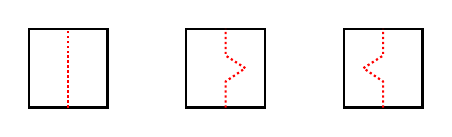
\begin{tikzpicture}
    %
    \cellF{0}{0}{1}{1}
    %
    \draw[thick] (2, 0) rectangle (3,1);
    \draw[red, thick, densely dotted] (3 * 0.5 + 2 * 0.5 , 0) -- (3 * 0.5 + 2 * 0.5 , 0.33) -- (3 * 0.75 + 2 * 0.25 , 0.5) -- (3 * 0.5 + 2 * 0.5 , 0.66) -- (3 * 0.5 + 2 * 0.5 , 1);
    %
    \draw[thick] (4, 0) rectangle (5,1);
    \draw[red, thick, densely dotted] (5 * 0.5 + 4 * 0.5 , 0) -- (5 * 0.5 + 4 * 0.5 , 0.33) -- (5 * 0.25 + 4 * 0.75 , 0.5) -- (5 * 0.5 + 4 * 0.5 , 0.66) -- (5 * 0.5 + 4 * 0.5 , 1);
\end{tikzpicture} 
\par\end{centering}
\caption{Various tiles that connect the top and bottom midpoints}
\label{fig: various top bottom tiles} 
\end{figure}

\noindent To count polygon mosaics in this new tile set, take $v$
such that $\begin{smallmatrix}0 & 1\\
1 & 0
\end{smallmatrix}$ and $\begin{smallmatrix}1 & 0\\
0 & 1
\end{smallmatrix}$ map to $0$, $\begin{smallmatrix}0 & 1\\
0 & 1
\end{smallmatrix}$ and $\begin{smallmatrix}1 & 0\\
1 & 0
\end{smallmatrix}$ map to $3$, and all other cells map to $1$. To count polygon free
mosaics, take $v$ that maps $\begin{smallmatrix}0 & 1\\
1 & 0
\end{smallmatrix}$ and $\begin{smallmatrix}1 & 0\\
0 & 1
\end{smallmatrix}$ to $0$, $\begin{smallmatrix}0 & 1\\
0 & 1
\end{smallmatrix}$ and $\begin{smallmatrix}1 & 0\\
1 & 0
\end{smallmatrix}$ to $3$, $\begin{smallmatrix}0 & 0\\
0 & 0
\end{smallmatrix}$ and $\begin{smallmatrix}1 & 1\\
1 & 1
\end{smallmatrix}$ to $9$, $\begin{smallmatrix}0 & 0\\
1 & 0
\end{smallmatrix}$ and $\begin{smallmatrix}1 & 0\\
1 & 1
\end{smallmatrix}$ to $-1$, and map the eight remaining cells to $1$.

One could also construct a tile set with both styles of tiles in Figure
\ref{fig:tile styles}. If this is done for each tile that joins adjacent
sides of the unit square, then to count polygon mosaics take $v$
such that $\begin{smallmatrix}0 & 1\\
1 & 0
\end{smallmatrix}$ and $\begin{smallmatrix}1 & 0\\
0 & 1
\end{smallmatrix}$ map to $0$, $\begin{smallmatrix}0 & 1\\
0 & 1
\end{smallmatrix}$, $\begin{smallmatrix}1 & 0\\
1 & 0
\end{smallmatrix}$, $\begin{smallmatrix}0 & 0\\
1 & 1
\end{smallmatrix},\begin{smallmatrix}1 & 1\\
0 & 0
\end{smallmatrix},\begin{smallmatrix}0 & 0\\
0 & 0
\end{smallmatrix}$, and $\begin{smallmatrix}1 & 1\\
1 & 1
\end{smallmatrix}$ map to $1$, and all other cells map to $2$. To count polygon free
mosaics, take $v$ that maps $\begin{smallmatrix}0 & 1\\
1 & 0
\end{smallmatrix}$ and $\begin{smallmatrix}1 & 0\\
0 & 1
\end{smallmatrix}$ to $0$, $\begin{smallmatrix}0 & 1\\
0 & 1
\end{smallmatrix}$, $\begin{smallmatrix}1 & 0\\
1 & 0
\end{smallmatrix}$, $\begin{smallmatrix}0 & 0\\
1 & 1
\end{smallmatrix}$, and $\begin{smallmatrix}1 & 1\\
0 & 0
\end{smallmatrix}$ map to $1$, $\begin{smallmatrix}0 & 0\\
0 & 0
\end{smallmatrix}$ and $\begin{smallmatrix}1 & 1\\
1 & 1
\end{smallmatrix}$ to $11$, $\begin{smallmatrix}0 & 0\\
1 & 0
\end{smallmatrix}$ and $\begin{smallmatrix}1 & 0\\
1 & 1
\end{smallmatrix}$ to $-2$, and map the six remaining cells to $2$. 

\noindent\textbf{The Lomonaco and Kauffman tile set.} Let us explore
what we can do with the Lomonaco and Kauffman tile set of Figure~\ref{fig: lk tile set}.
First we consider using only the first eight tiles, i.e., our usual
seven tiles of Figure~\ref{fig:tile set} plus the tile that connects
the top and left edges and also the bottom and right edges. Here we
use ``new polygon mosaic'' in this more general sense, i.e., mosaics
in which each tile is one of these eight type and in which every line
segment is part of a polygon. Our $\mathscr{L}$, as already defined,
extends to these new polygon mosaics, with the same reasoning showing
that $\mathscr{L}$ now gives a bijection, except from the set of
$\left(m,n\right)$ new polygon mosaics to the set of $\left(m,n\right)$
framed lattices, as opposed to $\left(m,n\right)$ proper lattices.
There are $2^{\left(m-1\right)\left(n-1\right)}$ $\left(m,n\right)$
polygon mosaics, which we can see either by directly counting the
number of $\left(m,n\right)$ proper lattices or by computing $\sum_{\ell}v\left(\ell\right)$
using the cell product function $v$ that maps all cells to $1$.
From here, we can easily count the number of knot mosaics by simply
adding tile variations. We can uniquely get any knot mosaic by taking
a new polygon mosaic and, wherever the eighth tile appears, use any
of the last four tiles. Therefore, we can count the number of knot
mosaics we use the cell product function that maps $\begin{smallmatrix}0 & 1\\
1 & 0
\end{smallmatrix}$ and $\begin{smallmatrix}1 & 0\\
0 & 1
\end{smallmatrix}$ to $4$, and maps the fourteen remaining cells to $1$. Calculating
in this way gives exactly the same number of knot mosaics as calculating
using Oh and colleagues' Theorem~1, their main result. We should
mention, however, that their calculated results, presented just after
their statement of Theorem~1, are not quite right. The $n=7$ case
is off by $2$ and each later line is off by more, though always by
a small percent. We speculate that the errors are due to the authors
using 64 bit fixed-precision arithmetic rather than arbitrary-precision
arithmetic.

We leave the readers with an open question, which is to count the
number of ``knot free mosaics,'' i.e., mosaics using the Lomonaco
and Kauffman tile set of Figure~\ref{fig: lk tile set} that contain
no knots. The techniques we used to count polygon free mosaics do
not seem to generalize to this question. One problem is that when
we interchange the eighth Lomonaco and Kauffman tile for one of the
remaining tiles, the number of knots can change. This suggests that
there may be no way to count the number of knots based on local information
in the manner of Proposition~\ref{prop: sign of v}.

\section{Acknowledgment}

The authors would like to thank Richard Schank for contributing ideas
toward the definition of $\mathscr{L}$ and ideas that led to Theorem~\ref{thm: m by n matrix}.

\newpage{}

% \newpage

\section{Appendix}
\begin{prop*}[The inclusion-exclusion principle]
For finite sets $A_{1},A_{2},\dots,A_{M}$, 
\[
\left|\bigcup^{M}_{j=1}A_{j}\right|=\sum_{\varnothing\neq I\subseteq\left\{ 1,2,\dots,M\right\} }\left(-1\right)^{\left|I\right|-1}\left|\bigcap_{j\in I}A_{j}\right|.
\]
\end{prop*}
\begin{proof}
The $M=1$ case is trivial, and $M=2$ case is the familiar and easily
justified statement that $\left|A_{1}\cup A_{2}\right|=\left|A_{1}\right|+\left|A_{2}\right|-\left|A_{1}\cap A_{2}\right|$.
We proceed inductively, so for $M\ge3$, assume the result for $M-1$
sets, and let us prove it for $M$ sets. We split up the sum on the
right of our desired equation into sets $I$ that do not contain $M$
and those that do. By our inductive hypothesis, the first sum equals
$\left|\bigcup^{M-1}_{j=1}A_{j}\right|$. The second sum is $\sum_{\left\{ M\right\} \subseteq I\subseteq\left\{ 1,2,\dots,M\right\} }\left(-1\right)^{\left|I\right|-1}\left|\bigcap_{j\in I}A_{j}\right|$,
which we rewrite by separating the $I=\left\{ M\right\} $ term and
reindexing the rest using $J=I\setminus\left\{ M\right\} $ to get
\[
\left|A_{M}\right|-\sum_{\varnothing\neq J\subseteq\{1,2,\dots,M-1\}}\left(-1\right)^{\left|J\right|-1}\left|\bigcap_{j\in J}\left(A_{j}\cap A_{M}\right)\right|.
\]
Again using our inductive hypothesis, this final sum equals $\left|\bigcup^{M-1}_{j=1}\left(A_{j}\cap A_{M}\right)\right|=\left|\left(\bigcup^{M-1}_{j=1}A_{j}\right)\cap A_{M}\right|.$
The entire right side of our desired equation therefore equals $\left|\bigcup^{M-1}_{j=1}A_{j}\right|+|A_{M}|-\left|\left(\bigcup^{M-1}_{j=1}A_{j}\right)\cap A_{M}\right|.$
By the $M=2$ case, this is $\left|\bigcup^{M}_{j=1}A_{j}\right|$,
as desired. 
\end{proof}


\end{document}
